\subsection{Python: A language, not a program}


\begin{frame}[plain]
	\makebox[\columnwidth]{
		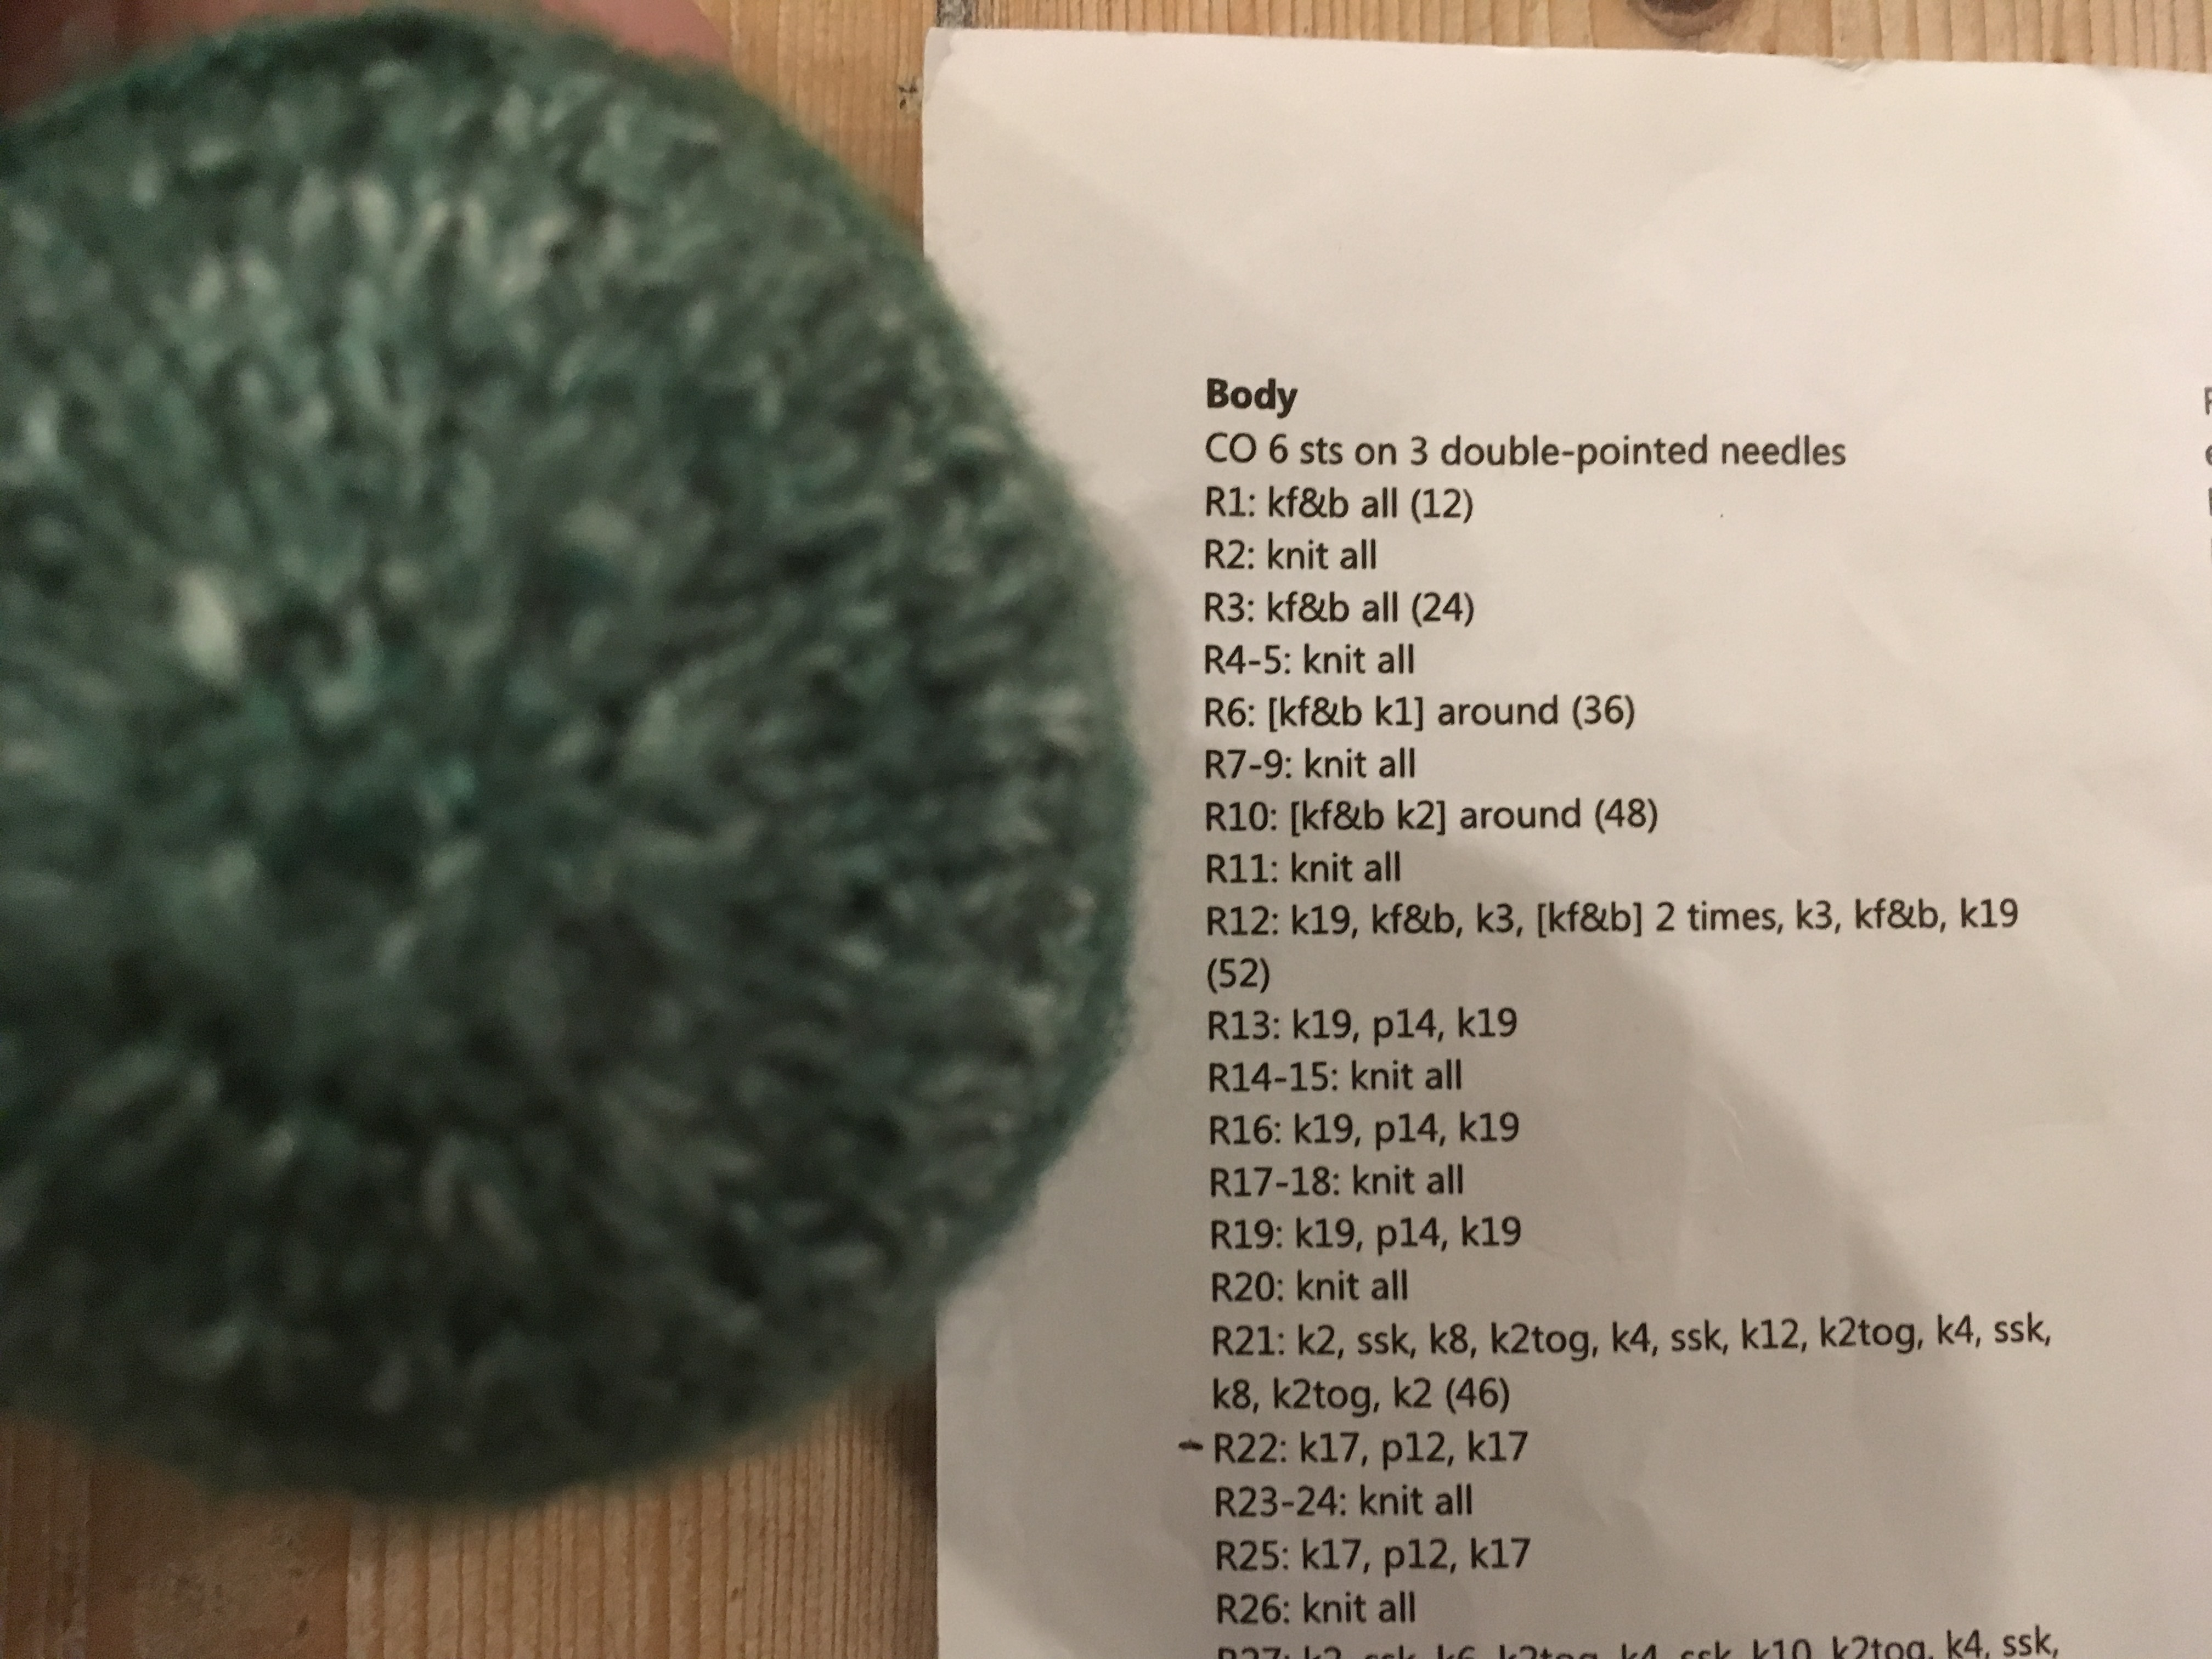
\includegraphics[width=\columnwidth,height=\paperheight,keepaspectratio]{knitting.jpg}}
	\footnotesize{An algorithm in a language that's a bit harder (I think) than Python}
\end{frame}



\begin{frame}{Python}
	\begin{block}{What?}<1->
		\begin{itemize}
			\item A language, not a specific program
			\item Huge advantage: flexibility, portability
			\item One of \emph{the} languages for CCS. \tiny{(The other one is R.)}
		\end{itemize}
	\end{block}
	
	\begin{block}{Which version?}<2->
		We use Python 3. (I use 3.8.10 right now, but with anything above 3.6 you're probably fine)\\ 
		You may occasionally still encounter Python2-code. One difference: In Python 2, you write {\tt print "Hi"} instead of {\tt print ("Hi")}.\\
	\end{block}
\end{frame}


\subsection{Python versus R}
\begin{frame}{Should I use Python or R?}
	\begin{itemize}
		\item For some people, an almost religious debate (but that's stupid!)
		\item Different history: R comes from math and statistics, Python from computer science
		\item Different user communities: statisticians: R, linguists: Python; most of industry: Python
		\item Nowadays (unlike some years ago), most things that are relevant to us can be done in \emph{both} languages.
	\end{itemize}
\pause
\textcolor{orange}{\textbf{Specialize in one language, but have a basic understanding of both!}}
\end{frame}


\begin{frame}{Should I use Python or R?}
	\begin{block}{For those of you who know R}
		You will notice a few things:
		\begin{itemize}[<+>]
			\item R ``abstracts away'' more stuff; in Python, you need to be a bit more explicit
			\item In R, (almost) everything is a dataframe or a vector, in Python not
			\item There is a big difference between applying a function to a single value or a whole ``column'' in Python
			\item In Python, we start counting with 0 (not 1)
		\end{itemize}

	\end{block}
\end{frame}


\begin{frame}{Should I use Python or R?}
	\begin{block}{For those of you who know R}
		You will notice a few things:
		\begin{itemize}[<+>]
			\item Typical ``user level'' R-code often is essentially written as consecutive commands: line for line. Structuring the code using typical programming constructs (writing own functions, using control strucutures) is not considered ``pro'' use (like in R), but \emph{the} way to work in Python.
			\item Python likes object orientation, R likes functions and pipelines
		\end{itemize}
		
	\end{block}
\end{frame}



\begin{frame}{Why do we use Python in this course?}
\begin{itemize}
	\item Python is a general programming language, R is a domain-specific one (it's meant for stats).
	\item The course is on ACA, and the closely related computational linguistics community uses Python.
	\item Python is \emph{much} better equipped for machine learning (and R for traditional stats, but that's not our focus).
	\item Web scraping is possible in R, but typically done in Python.
	\item If you know Python, you can probably learn many other languages quite quickly (including R). That's a bit more difficult coming from R.
\end{itemize}
	
\end{frame}



\begin{frame}{You can build \emph{anything}, including a live news aggregator!} 
	Beyond the scope of this course, but this was a Master thesis \parencite{3bij3}:
	\makebox[\columnwidth]{
		\includegraphics[width=\columnwidth,height=\paperheight,keepaspectratio]{3bij3article.png}}
\end{frame}


\begin{frame}[plain]
	\makebox[\columnwidth]{
		\includegraphics[width=\columnwidth,height=\paperheight,keepaspectratio]{3bij3article2.png}}
\end{frame}

\subsection{What do we need to write Python programs?}

\begin{frame}{1. A Python interpreter}
A Python interpreter -- a program that ``understands'' Python and translates it into low-level commands that your computer executes.

Type \texttt{python3} in your operating system's command line:

	\makebox[\columnwidth]{
	\includegraphics[width=.8\columnwidth,keepaspectratio]{repl.png}}
That's also called a Read-Evaluate-Print-Loop (REPL)
\end{frame}

\begin{frame}{2. Some more comfort}
\begin{itemize}[<+->]
	\item Starting an interpreter like this useful for quick try-outs, but not really a way to write full programs
	\item You can write them in a (good) text editor (Atom, Sublime, Notepad++, geany, emacs, vi) -- that's how it has historically been done and still a good skill to have
	\item But there are also \emph{Integrated Development Environments} (IDEs) that integrate an editor and an interpreter and offer a lot of extra funcitonality
	\item We will mainly work with Jupyter (which is tailored to data analyst's needs), but you you can consider checking out PyCharm or Visual Studio Code (both used by professional programmers) or Spyder (for those who like RStudio)
\end{itemize}
\end{frame}

\begin{frame}{3. Additional modules}
	\begin{itemize}
		\item A great advantage of Python are the many packages to extend it. 
		\item You can install them using a command called \texttt{pip}
		\item Alternatively, the Anaconda distribution already comes with most (but probably not all) you'll need pre-installed.
	\end{itemize}
\end{frame}

\question{You see why I talked about the difference between monolitic software like SPSS and the ``a language, not a program''-notion here?}